%%%%%%
%
% $Autor: Wings $
% $Datum: 2020-01-18 11:15:45Z $
% $Pfad: WuSt/Skript/Produktspezifikation/powerpoint/ImageProcessing.tex $
% $Version: 4620 $
%
%%%%%%

%Quelle: https://towardsdatascience.com/from-lenet-to-efficientnet-the-evolution-of-cnns-3a57eb34672f


%\begin{figure}[!h]
%    %\begin{subfigure}[h]{0.4\linewidth}
%%todo Eigene Bilder    
%    \includegraphics[width=0.7\textwidth]{CoralTPU/Concept/dogs}
%\end{figure}
% {\tiny Quelle: \href{https://machinelearners.net/2017/08/23/predicting-bitcoins-value-using-convolution-neural-networks-long-short-term-memory-cells/}{Vaibhav Sharma : Predicting bitcoin’s Value Using Convolution neural networks \& Long short term memory cells!} \cite{Sharma:2017}}



%todo 
%\url{https://machinelearners.net/2017/08/23/predicting-bitcoins-value-using-convolution-neural-networks-long-short-term-memory-cells/}



%Inspired n from the  program image classification on coral Usb accleator coded by Adrian, a similar procedure was followed to program this  image classification program .\newline
\section{Convolution Neural Network}

One focus for machine learning is the interpretation of images. Two cases must be distinguished here

\begin{enumerate}
    \item Object detection\index{Object detection}
    \item Image classification.\index{Image classification}
    
\end{enumerate}. 

When detecting objects, an image is examined to see if one or more objects can be identified. If an object is detected, the coordinates of the surrounding rectangle and the class or classes of the object are returned with a respective probability. With the segmentation\index{segmentation}, instead of the coordinates of the surrounding rectangle, a polygon course is returned that surrounds the object. In contrast, when classifying an image, a description of the image is searched for. In both cases \ac{cnn} are commonly used and are described in the following section. 

A \ac{cnn} expects an image as input information. If images do not contain colour information, they are represented as matrices whose number of columns and rows correspond to the number of pixels in width and height. In the case that an image contains colour information, such a matrix is created for each colour. In this case, one speaks of colour channel or simply of channel{index{channel}.
	
	
\ac{cnn} is a commonly used shift-invariant method for extracting adaptive features. Its success has contributed to the popularity of machine learning. In its history, its architectures have undergone a great evolution.\index{Alom:2018} Some well-known architectures are now described.    
	
\subsection{CNN Architectures}


\subsection{LeNet\index{LeNet}}

In 1998, the CNN architecture LeNet was the first CNN architecture to use back-propagation for practical applications. It thus transported Deep Learning from theory to practice. LeNet was used for handwritten digit recognition and was able to outperform all other existing methods. The architecture was very simple with only 5 layers consisting of $5\times 5$ convolutions and $2\times 2$ max-pooling, but paved the way for better and more complex models. \cite{LeCun:1998} The listing of elements in Table~\ref{Concept:LeNet} contains several points that will be described later.



% https://www.kaggle.com/blurredmachine/lenet-architecture-a-complete-guide


\begin{figure}
  \includegraphics[page=7,width=0.9\textwidth,viewport=20 600 560 740,clip]{../../MLbib/CNN/Lecun98.pdf}

  \caption{Struktur der CNN-Architektur gemäß LeCun et.al. \cite{LeCun:1998}}\label{Concept:LeNet}
\end{figure}

\begin{table}
  \begin{tabular}{ccc ccc c}
  	\multicolumn{2}{c}{\textbf{Layer}} & \textbf{\begin{tabular}{c}Feature\\ Map \end{tabular}} & \textbf{Size} & \textbf{\begin{tabular}{c} Kernel \\Size\\ \end{tabular}} & \textbf{Stride} & \textbf{\begin{tabular}{c}Acti- \\vation \\function \end{tabular}}  \\ \hline
  	Input   & Image            &   1 & $32\times 32$ &            - & - & - \\
  	1        & Convolution     &   6 & $28\times 28$ &  $5\times 5$ & 1 & $\tanh$ \\  
  	2        & \begin{tabular}{c}Average\\ Pooling  \end{tabular} &   6 & $14\times 14$ &  $2\times 2$ & 2 & $\tanh$ \\  
  	3        & Convolution     &  16 & $10\times 10$ &  $5\times 5$ & 1 & $\tanh$ \\  
    4        & \begin{tabular}{c}Average\\ Pooling  \end{tabular} &  16 &   $5\times 5$ &  $2\times 2$ & 2 & $\tanh$ \\  
  	5        & Convolution     & 120 &   $1\times 1$ &  $5\times 5$ & 1 & $\tanh$ \\  
  	6        & \begin{tabular}{c}Neural\\ Network  \end{tabular} &   - &          $84$ &    -         & - & $\tanh$ \\  
  	Ausgabe  & \begin{tabular}{c}Neural\\ Network  \end{tabular}  &   - &          $10$ &    -         & - & softmax \\  
  \end{tabular}  		
  \caption{Structural elements of LeNet}
%  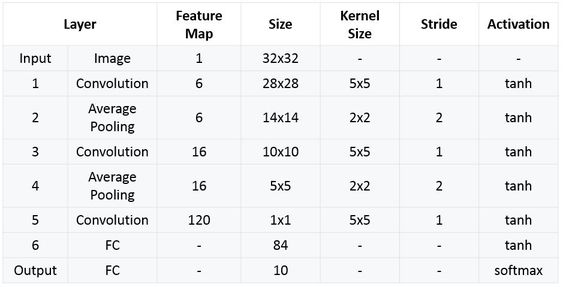
\includegraphics[scale=0.7]{Bilder/CNN/LeNetStructure}

\end{table}

  


\subsection{AlexNet\index{AlexNet}} 

The AlexNet architecture was the first to use CNN models implemented on \ac{gpu}s.  In 2012, this really connected the growing computing power with Deep Learning. AlexNet is significantly deeper and more complex than LeNet They also started using ReLU activations instead of sigmoid or tanh, which helped train better models. AlexNet not only won the 2012 ImageNet classification competition, but beat the runner-up by a margin that suddenly made non-neural models almost obsolete. \cite{Krizhevsky:2012}

%https://www.kaggle.com/blurredmachine/alexnet-architecture-a-complete-guide


\subsection{InceptionNet\index{InceptionNet}}


The architecture InceptionNet\index{InceptionNet} used the increased possibilities of the hardware. The architecture was again much deeper and richer in parameters than the existing models. To deal with the problem of training deeper models, they used the idea of multiple auxiliary classifiers present between the model to prevent the gradient from breaking. One of their ideas was to use kernels of different sizes in parallel, thus increasing the width of the model instead of the depth. This allows such an architecture to extract both larger and smaller features simultaneously. \cite{Szegedy:2014}


\subsection{VGG\index{VGG}}

Many architectures tried to achieve better results by using larger convolution kernels. For example, the architecture AlexNet\index{AlexNet} uses cores of size $11 \times 11$, among others. The architecture VGG\index{VGG} took the path of using several cores of size $3\times 3$ in succession and more non-linearities in the form of activation functions. This again improved the results. \cite{Zhang:2015,Simonyan:2015}

\subsection{Residual Neural Network (ResNet)\index{ResNet}}

% https://towardsdatascience.com/an-overview-of-resnet-and-its-variants-5281e2f56035
The deeper the architectures became, the more often the problem occurred during training that the amount of the gradient became too small. The backpropagation\index{backpropagation} then aborted and the parameters could not be determined. In the \ac{resnets} architecture, to prevent the problem, residual or shortcut links were introduced to create alternative paths for the gradient to skip the middle layers and directly reach the initial layers. In this way, the authors were able to train extremely deep models that previously did not perform well. It is now common practice to have residual connections in modern CNN architectures. \cite{He:2016}




\subsection{MobileNet \& MobileNetV2\index{MobileNet}\index{MobileNetV2}} %: Moving towards edge-friendly models

The MobileNet architecture is designed for edge computers and smart phones that are limited in memory and computing power. This has opened up a large field of new applications. This is in contrast to the previous strategy of increasing the size of architectures by introducing separable convolutions. In simple terms, a two-dimensional convolutional kernel is split into two separate convolutions, namely the depth convolution, which is responsible for collecting the spatial information for each individual channel, and the point convolution, which is responsible for the interaction between the different channels. Later, MobileNetV2 was also introduced with residual connections and other optimisations in the architecture to further reduce the model size. \cite{Howard:2017,MobileNet:2018}

\subsection{EfficientNet\index{EfficientNet}} %: Squeeze and Excitation layers

The architecture is the result of considering that the various architectures to date, focus on either performance or computational efficiency. The authors of \cite{Tan:2020} claimed that these two problems can be solved by similar architectures. They proposed a common CNN skeleton architecture and three parameters, namely the width, the depth and the resolution. The width of the model refers to the number of channels present in the different layers, the depth refers to the number of layers in the model and the resolution refers to the size of the input image to the model. They claimed that by keeping all these parameters small, one can create a competitive yet computationally efficient CNN model. On the other hand, by increasing the value of these parameters, one can create a model that is designed for accuracy.

%
%Obwohl Squeeze- und Excitation-Schichten bereits früher vorgeschlagen wurden, waren sie die ersten, die diese Idee in Mainstream-CNNs einführten. S\& E-Schichten erzeugen kanalübergreifende Interaktionen, die invariant gegenüber räumlichen Informationen sind. Dies kann genutzt werden, um den Einfluss von weniger wichtigen Kanälen zu verringern. Sie führten auch die neu vorgeschlagene Swish-Aktivierung anstelle von ReLU ein, was ein wichtiger Faktor für die Leistungsverbesserung war. EfficientNets sind derzeit die leistungsstärksten Klassifikationsmodelle unter verschiedenen Kategorien der Verfügbarkeit von Rechenressourcen.

\subsection{General Structure}



In the description of the architectures, some elements necessary for the construction were mentioned. All building blocks can be listed as follows:

\begin{itemize}
	\item Convolutional layer (convolution)
	\item Activation function
	\item Pooling
	\item Flattening
	\item Neural network
\end{itemize}

Each component is characterised by further variables. The combination and configuration of the building blocks are summarised in the so-called hyperparameters. By specifying the hyperparameter\index{hyperparameter}, the architecture and the number of parameters is determined. For example, in a neural network, the hyperparameters\index{hyperparameters} are the number of layers, the number of neurons per layer and the determination of the activation functions. If the number of all neurons is now determined, this results in the number of parameters that are determined during the training.

In the table~\ref{concept:Parameter} some architectures are compared. The table indicates the number of parameters to be trained.  If an image is classified, the models give different possibilities and assign a probability to them. The accuracy now indicates the percentage with which the image matches the prediction with the highest probability. For this purpose, the models were trained and validated with the ImageNet\index{ImageNet}. 




 \begin{table}
   \begin{tabular}{lllrc}
     Model             & Size   & Accuracy    & Parameter   & Depth \\ \hline
     VGG16             & 528 MB & 71{,}3\%    & 138.357.544 & 23 \\     
     VGG19             & 549 MB & 71{,}3\%    & 143.667.240 & 26 \\     
     ResNet-50         &  98 MB & 74{,}9\%    &  25.636.712 & 50 \\     
     ResNet-101        & 171 MB & 76{,}4\%    &  44.707.176 & 101 \\     
     ResNet-152        & 232 MB & 76{,}6\%    &  60.419.944 & 152 \\     
     InceptionV3       &  92 MB & 77{,}9\%    &  23,851,784 & 159 \\
     InceptionResNetV2 & 215 MB & 80{,}3\%    &  55,873,736 & 572 \\
%     NASNetMobile      &  23 MB & 74{,}4\%    &   5.326.716 & --\\
%     NASNetLarge       & 343 MB & 82{,}5\%    &  88.949.818 & --\\
     MobileNet         &  16 MB & 70,{4}\%    &   4.253.864 & 88 \\       
     MobileNetV2       &  14 MB & 71,{3}\%    &   3.538.984 & 88 \\       
    \end{tabular}
  \caption{Characteristics of different \ac{cnn} architectures\index{VGG}\index{ResNet}\index{Inception}\index{MonileNet}}\label{concept:Parameter}
 \end{table}
 
The individual building blocks are now described below.



\subsection{Input and Output}

When a model receives an image as input, fields with pixel values are transferred. The height, the width and the number of colour channels determine the size of the fields. The elements of the fields then contain values between zero and 255. This value is the intensity of the pixel. The model then determines probabilities of how to classify an image based on these fields. For example, the result could be that $81\%$ of the image is a turtle, $11\%$ is a gun and $8\%$ is a chocolate bar.


%todo Sichtbar machen der Filter, Lernen der Filter



\subsection{Convolution Layer}\label{subsec:conv2d}

In a convolution layer, the input data is modified by one or more filters. In image processing, this is the application of a defined set of filters to two-dimensional data.

The size of this filter is defined by the so-called kernel: a $3 \times 3$ kernel is represented by a $3 \times 3$ matrix. In order to be able to apply the filter, a range of pixel values is defined that has the same size; the pixel values are then also stored in a matrix. By convolution of the matrix, as shown in the equation~\ref{concept:convolutionMatrix}, a value is assigned to the matrix and the filter. 
    
   
    \begin{figure}
        
        $$A \ast C 
        =
        \left(
        \begin{matrix}
            a_{11} & a_{12} & a_{13}\\
            a_{21} & a_{22} & a_{23}\\
            a_{31} & a_{32} & a_{33}\\
        \end{matrix}
        \right)
        \ast
        \left(
        \begin{matrix}
            c_{11} & c_{12} & c_{13}\\
            c_{21} & c_{22} & c_{23}\\
            c_{31} & c_{32} & c_{33}\\
        \end{matrix}
        \right)
        = 
        \sum_{i=1}^3\sum_{j=1}^3  a_{ij} \cdot c_{ij}
        $$
        
        \caption{Definition of the convolution of two matrices}\label{concept:FaltungMatrix}
        
    \end{figure}
 
 To apply a filter, matrices must therefore be systematically selected from the pixel values. Since the dimension of a kernel is defined by an odd number $2n+1$, a surrounding matrix can be assigned to each pixel value that has a distance greater than $n$ from the edge. In the figure~\ref{concept:conv2d} such a situation is shown. The filter, labelled $C$ and coloured purple, has a dimension of $3 \times 3$. In the matrix $A$, the field of pixel values, a region is coloured red. In the middle is the pixel from the fifth column and the second row. The filter is now applied to this area of the matrix $A$. The result is then entered into the matrix $A\ast C$. In this case the value is $4$ and marked green.
 
 
 A filter is now moved step by step over the data.  The filter can be applied to any pixel value that is far enough from the edge, or individual pixels can be skipped. This is defined by the step size, also called stride. With a step size of one, every pixel is used. To reduce the output size, stride sizes larger than one can be used; it is also possible to set different stride sizes for width and height. If a step size of $2$ is specified in both directions, the amount of data has been reduced to $25\%$. \cite{Dumoulin:2016}
 
 In the figure~\ref{concept:conv2d}, the input matrix is a $7\times 7$ matrix. Since a step size of one is applied here, the result is a $5\times 5$ matrix.
 
 Often an activation function is applied to each result.
     
    \begin{figure}[htb]
        
       
        \centering
        \begin{tikzpicture}
            % SOURCE: https://github.com/PetarV-/TikZ/blob/master/2D%20Convolution/2d_convolution.tex
            \matrix (mtr) [matrix of nodes,row sep=-\pgflinewidth, nodes={draw}]
            {
                0 & 1 & 1 & |[fill=red!20]| 1 & |[fill=red!20]| 0 & |[fill=red!20]| 0 & 0\\
                0 & 0 & 1 & |[fill=red!20]| 1 & |[fill=red!20]| 1 & |[fill=red!20]| 0 & 0\\
                0 & 0 & 0 & |[fill=red!20]| 1 & |[fill=red!20]| 1 & |[fill=red!20]| 1 & 0\\
                0 & 0 & 0 & 1 & 1 & 0 & 0\\
                0 & 0 & 1 & 1 & 0 & 0 & 0\\
                0 & 1 & 1 & 0 & 0 & 0 & 0\\
                1 & 1 & 0 & 0 & 0 & 0 & 0\\
            };
            
            \draw[very thick, red!20] (mtr-1-4.north west) rectangle (mtr-3-6.south east);
            
            \node [below= of mtr-5-4.south] (lm) {$\mathbf{A}$};
            
            \node[right = 0.2em of mtr] (str) {$*$};
            
            \node (ast2) at (2,-2) {$\mathbf{*}$};
            \node (ast2) at (4,-2) {$\mathbf{=}$};
            
            \matrix (K) [right=0.2em of str,matrix of nodes,row sep=-\pgflinewidth, nodes={draw, fill=blue!20}]
            {
                1 & 0 & 1 \\
                0 & 1 & 0 \\
                1 & 0 & 1 \\
            };
            \node [below = of K-3-2.south] (lk) {$\mathbf{C}$};
            
            \node [right = 0.2em of K] (eq) {$=$};
            
            \matrix (ret) [right=0.2em of eq,matrix of nodes,row sep=-\pgflinewidth, nodes={draw}]
            {
                1 & 4 & 3 & |[fill=green!20]| 4 & 1\\
                1 & 2 & 4 & 3 & 3\\
                1 & 2 & 3 & 4 & 1\\
                1 & 3 & 3 & 1 & 1\\
                3 & 3 & 1 & 1 & 0\\
            };
            \node [below = of ret-4-3.south] (lim) {$\mathbf{A} \ast  \mathbf{C}$};
            
            \draw[very thick, green!20] (ret-1-4.north west) rectangle (ret-1-4.south east);
            
            \draw[densely dotted, blue!30, thick] (mtr-1-4.north west) -- (K-1-1.north west);
            \draw[densely dotted, blue!30, thick] (mtr-3-4.south west) -- (K-3-1.south west);
            \draw[densely dotted, blue!30, thick] (mtr-1-6.north east) -- (K-1-3.north east);
            \draw[densely dotted, blue!30, thick] (mtr-3-6.south east) -- (K-3-3.south east);
            
            \draw[densely dotted, green!30, thick] (ret-1-4.north west) -- (K-1-1.north west);
            \draw[densely dotted, green!30, thick] (ret-1-4.south west) -- (K-3-1.south west);
            \draw[densely dotted, green!30, thick] (ret-1-4.north east) -- (K-1-3.north east);
            \draw[densely dotted, green!30, thick] (ret-1-4.south east) -- (K-3-3.south east);
            
            \matrix (K) [right=0.2em of str,matrix of nodes,row sep=-\pgflinewidth, nodes={draw, fill=blue!20}]
            {
                1 & 0 & 1 \\
                0 & 1 & 0 \\
                1 & 0 & 1 \\
            };
            
            \draw[very thick, blue!20] (K-1-1.north west) rectangle (K-3-3.south east);
            
            \node[anchor=south east, inner sep=0.01em, blue!20] at (mtr-1-4.south east) (xx) {\scalebox{.5}{$\times 1$}};
            \node[anchor=south east, inner sep=0.01em, blue!20] at (mtr-1-5.south east) (xx) {\scalebox{.5}{$\times 0$}};
            \node[anchor=south east, inner sep=0.01em, blue!20] at (mtr-1-6.south east) (xx) {\scalebox{.5}{$\times 1$}};
            \node[anchor=south east, inner sep=0.01em, blue!20] at (mtr-2-4.south east) (xx) {\scalebox{.5}{$\times 0$}};
            \node[anchor=south east, inner sep=0.01em, blue!20] at (mtr-2-5.south east) (xx) {\scalebox{.5}{$\times 1$}};
            \node[anchor=south east, inner sep=0.01em, blue!20] at (mtr-2-6.south east) (xx) {\scalebox{.5}{$\times 0$}};
            \node[anchor=south east, inner sep=0.01em, blue!20] at (mtr-3-4.south east) (xx) {\scalebox{.5}{$\times 1$}};
            \node[anchor=south east, inner sep=0.01em, blue!20] at (mtr-3-5.south east) (xx) {\scalebox{.5}{$\times 0$}};
            \node[anchor=south east, inner sep=0.01em, blue!20] at (mtr-3-6.south east) (xx) {\scalebox{.5}{$\times 1$}};	
        \end{tikzpicture}
        \caption{Convolution layer with $3 \times 3$ kernel and stride (1, 1)}
        \label{concept:conv2d}
        
    \end{figure}
    
When defining the filters, make sure that the filter is defined for each channel.
To capture the features in an image, the values in the filter must match the structure of the original pixel values of the image. Basically, if there is a shape in the input image that generally resembles the curve that this filter represents, then the convolution will result in a large value.

As a rule, several filters are used in parallel. The result is so-called feature maps\index{feature maps}. Further convolution layers are then applied to this result, which in turn generate feature maps. 


\subsubsection{Feature Identification}

A convolution is defined by filters. Each filter can be interpreted as an identifier of features. Features are, for example, edges, colours or even curves. For example, the $7\times 7$ filter is considered:

$$\left(
\begin{array}{ccc ccc c}
    0 & 0 & 0 &  0 & 0  & 50 & 0 \\
    0 & 0 & 0 &  0 & 50 &  0 & 0 \\
    0 & 0 & 0 & 50 &  0 &  0 & 0 \\
    0 & 0 & 0 & 50 &  0 &  0 & 0 \\
    0 & 0 & 0 & 50 &  0 &  0 & 0 \\
    0 & 0 & 0 & 50 &  0 &  0 & 0 \\
    0 & 0 & 0 &  0 &  0 &  0 & 0 \\
\end{array}
\right)
$$  

This filter can also be visualised as images:

%todo Image generieren



To demonstrate the effect of the filter, a sample image~\ref{concept:FilterCat} is considered:


\begin{figure}
  \centering    

%todo Eigenes Bild
  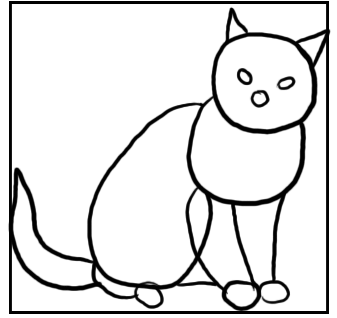
\includegraphics[scale=0.3]{CNN/cat}
    
  \caption{Beispielanwendung für einen Filter und ein Ausschnitt}\label{concept:FilterCat}
\end{figure}

In the example image~\ref{concept:FilterCat} a section is marked to which the filter is applied. 



$$
\left(
\begin{array}{ccc ccc c}
    0 & 0 & 0 &  0 & 0  &  0 & 30 \\
    0 & 0 & 0 &  0 & 80 & 80 & 80 \\
    0 & 0 & 0 & 30 & 80 &  0 &  0 \\
    0 & 0 & 0 & 80 & 80 &  0 &  0 \\
    0 & 0 & 0 & 80 & 80 &  0 &  0 \\
    0 & 0 & 0 & 80 & 80 &  0 &  0 \\
    0 & 0 & 0 & 80 & 80 &  0 &  0 \\
\end{array}
\right)
\star
\left(
\begin{array}{ccc ccc c}
    0 & 0 & 0 &  0 & 0  & 50 & 0 \\
    0 & 0 & 0 &  0 & 50 &  0 & 0 \\
    0 & 0 & 0 & 50 &  0 &  0 & 0 \\
    0 & 0 & 0 & 50 &  0 &  0 & 0 \\
    0 & 0 & 0 & 50 &  0 &  0 & 0 \\
    0 & 0 & 0 & 50 &  0 &  0 & 0 \\
    0 & 0 & 0 &  0 &  0 &  0 & 0 \\
\end{array}
\right)$$

$$
=
\left(
\begin{array}{ccc ccc c}
    0 & 0 & 0 &  0 & 0  &  0 & 30 \\
    0 & 0 & 0 &  0 & 80 & 80 & 80 \\
    0 & 0 & 0 & 30 & 80 &  0 &  0 \\
    0 & 0 & 0 & 80 & 80 &  0 &  0 \\
    0 & 0 & 0 & 80 & 80 &  0 &  0 \\
    0 & 0 & 0 & 80 & 80 &  0 &  0 \\
    0 & 0 & 0 & 80 & 80 &  0 &  0 \\
\end{array}
\right)
$$  

The basic property of filters is clarified. If there is a shape in the input image that generally resembles the filter, then large values result. A probability is then assigned via the activation function. Various filters are then defined and applied in the convolution layer. The result is then the feature map. The figure~\ref{concept:FilterVis} shows some examples of concrete visualisations of filters of the first convolutional layer of a trained network. 


\begin{figure}[!h]
  \centering
    %\begin{subfigure}[h]{0.4\linewidth}
%  \includegraphics[width=0.7\textwidth]{CoralTPU/Concept/FirstLayers}
  
  \includegraphics[viewport=0 350 280 480,clip,page=2,width=0.7\textwidth]{../../MLbib/CNN/08663285.pdf}
    
  \caption{Visualisation of filters of a trained network \cite{Lu:2019,Shang:2016}}\label{concept:FilterVis}
\end{figure}


\subsubsection{Edge Detection}

Suitable filters can also be defined for edge detection. The filter


$$\left(
\begin{array}{ccc}
    1 & 0 & -1 \\
    1 & 0 & -1 \\
    1 & 0 & -1 \\
\end{array}
\right)
$$

can be used for a vertical edge detection, whereas the filter 


$$\left(
\begin{array}{ccc}
    1 &  1 &  1 \\
    0 &  0 &  0 \\
    -1 & -1 & -1 \\
\end{array}
\right)
$$

can be used for a horizontal one. Both filters are now applied to a vertical edge.


\begin{figure}
$$
\left(
\begin{array}{ccc ccc}
    10 & 10 & 10 & 0 & 0 & 0 \\
    10 & 10 & 10 & 0 & 0 & 0 \\
    10 & 10 & 10 & 0 & 0 & 0 \\
    10 & 10 & 10 & 0 & 0 & 0 \\
    10 & 10 & 10 & 0 & 0 & 0 \\
    10 & 10 & 10 & 0 & 0 & 0 \\
\end{array}
\right)
\ast
\left(
\begin{array}{ccc}
    1 & 0 & -1 \\
    1 & 0 & -1 \\
    1 & 0 & -1 \\
\end{array}
\right)
=
\left(
\begin{array}{cccc}
    0 & 30 & 30 & 0 \\
    0 & 30 & 30 & 0 \\
    0 & 30 & 30 & 0 \\
    0 & 30 & 30 & 0 \\
\end{array}
\right)
$$

$$
\left(
\begin{array}{ccc ccc}
    10 & 10 & 10 & 0 & 0 & 0 \\
    10 & 10 & 10 & 0 & 0 & 0 \\
    10 & 10 & 10 & 0 & 0 & 0 \\
    10 & 10 & 10 & 0 & 0 & 0 \\
    10 & 10 & 10 & 0 & 0 & 0 \\
    10 & 10 & 10 & 0 & 0 & 0 \\
\end{array}
\right)
\ast
\left(
\begin{array}{ccc}
    1 &  1 &  1 \\
    0 &  0 &  0 \\
    -1 & -1 & -1 \\
\end{array}
\right)
=
\left(
\begin{array}{cccc}
    0 & 0 & 0 & 0 \\
    0 & 0 & 0 & 0 \\
    0 & 0 & 0 & 0 \\
    0 & 0 & 0 & 0 \\
\end{array}
\right)
$$
  \caption{Detection of vertical and horizontal edges}
\end{figure}

Edges can be present in any arrangement in images, edge detection must take this into account. That is, if a \ac{cnn} is trained, the filters evolve based on the given images. 



\subsection{Padding}

In the previous representation, filters could not be applied to boundary values. On the one hand, this means that information is not used, on the other hand, the size of the images is reduced each time the folding is applied. To prevent this, padding is applied. For a filter of dimension $(2n+1) \times (2m+1)$, the input image is padded with an additional border of size
$n$ and $m$. The additional values are each zero occupied.



\subsection{Activation function}\label{subsec:activation}

The activation function is applied to the respective output of a layer and determines how the output value should be interpreted by applying a defined function. Here, the respective input values, as well as a bias, are included in the calculation and determine whether the neuron is triggered \cite{Nwankpa:2018}. In this example, the \ac{relu} function is used for this: for input values less than or equal to zero, the function returns zero; for positive values, it behaves linearly \cite{Agarap:2018}. Thus, only positive values are returned (\cref{fig:relu}).

\begin{figure}
    \centering
    \begin{tikzpicture}
        \begin{axis}[
            domain=-5:5,
            axis equal,
            xmin=-5,
            xmax=5,
            axis y line=middle,
            axis x line=center,
            axis line style={->},
            xlabel={$x$},
            ylabel={$y$},
            xtick={-5,...,5},
            ytick={0,...,5},]
            \addplot+[mark=none,red,domain=-5:0] {0};
            \addplot+[mark=none,red,domain=0:5] {x};
        \end{axis}
    \end{tikzpicture}
    \caption{Representation of the ReLu activation function}
    \label{fig:relu}
\end{figure}

For example, an activation function can be applied after a convolution. This is shown in the equation~\ref{concept:ActivationMatrix}.


    \begin{figure}
    
    $$
      \ReLU(A) 
      = 
      \left(
        \begin{matrix}
          \ReLU(a_{11}+b) & \ReLU(a_{12} & \ldots & \ReLU(a_{1m}+b)\\
          \ReLU(a_{21}+b) & \ReLU(a_{22} & \ldots & \ReLU(a_{2m}+b)\\
             \vdots       & \ddots       &        &   \vdots \\
          \ReLU(a_{n1}+b) & \ReLU(a_{n2} & \ldots & \ReLU(a_{nm}+b)\\
    \end{matrix}
    \right)
    $$
    
    \caption{Application of an activation function with a bias $b \in \R$ to a matrix}\label{concept:AktivierungMatrix}
    
\end{figure}





\subsection{Pooling}


After the use of convolutional layers, pooling layers are often used in \ac{cnn} to reduce the size of the representation, to also speed up the calculations as well as to make some of the detection functions a bit more robust. A distinction is usually made between two pooling methods.

\begin{itemize}
  \item Max Pooling
  \item Average Pooling
\end{itemize}

In pooling, areas of a matrix are combined. The ranges are defined by two values $n$ and $m$. The ranges are submatrices of the matrix of size $n \times m$. A function is then applied to each submatrix.

In max-pooling, the maximum value of the submatrix is determined and entered as the result. In the case of average pooling, the average value of the matrix elements is determined instead of the maximum value and used further.


In the case of pooling, a window with a defined size is moved over the input matrix and the corresponding value within the window is taken over as a pooled value. The step size with which the window moves over the matrix is defined via a parameter \cite{Dumoulin:2016}. The default value corresponds to the size of the sub-matrix. An example is shown in the representation~\ref{fig:maxpooling2d}: a \twod{4}{4}-matrix is defined with size \PYTHON{pool\_size}  \twod{2}{2} and a step size \PYTHON{stride\_size} \twod{2}{2} processed. Since two values are combined into each dimension, the dimensions of the output matrix are halved in contrast to the input matrix. \cite{Britz:2015}

\begin{figure}[htb]
    \centering
    
    \def\yspacing{.75em}
    \begin{tikzpicture}[auto, node distance=0cm,>=latex']
        % Root folder blocks
        % Subfolder Blocks
        \node [smallblock] (bin) {2};
        \node [smallblock, below=of bin] (bin2) {0};
        \node [smallblock, right=of bin] (bin3) {0};
        \node [smallblock, right=of bin2] (bin4) {1};
        
        \node [smallblock, fill=blue!20, right=of bin3] (bin5) {1};
        \node [smallblock, fill=blue!20, below=of bin5] (bin6) {0};
        \node [smallblock, fill=blue!20, right=of bin5] (bin7) {1};
        \node [smallblock, fill=blue!20, right=of bin6] (bin8) {0};
        
        \node [smallblock, fill=green!20, below=of bin2] (bin9) {0};
        \node [smallblock, fill=green!20, below=of bin9] (bin10) {0};
        \node [smallblock, fill=green!20, right=of bin9] (bin11) {0};
        \node [smallblock, fill=green!20, right=of bin10] (bin12) {3};
        
        \node [smallblock, fill=yellow!20, right=of bin11] (bin13) {1};
        \node [smallblock, fill=yellow!20, below=of bin13] (bin14) {0};
        \node [smallblock, fill=yellow!20, right=of bin13] (bin15) {0};
        \node [smallblock, fill=yellow!20, right=of bin14] (bin16) {0};
        
        \node [smallblock, right=of bin8.east, xshift=10em] (res1) {2};
        \node [smallblock, fill=green!20, below=of res1] (res2) {3};
        \node [smallblock, fill=blue!20, right=of res1] (res3) {1};
        \node [smallblock, fill=yellow!20, right=of res2] (res4) {1};
        
        \draw [arrow] (bin8.south east)++(1em, 0) -- ($(res1.south west)+(-1em,0)$) node[midway, sloped, above] {\footnotesize pool\_size = (2,2)} node[midway, sloped, below] {\footnotesize stride = (2,2)};
    \end{tikzpicture}

    \bigskip
    
    \def\yspacing{.75em}
  \begin{tikzpicture}[auto, node distance=0cm,>=latex']
    % Root folder blocks
    % Subfolder Blocks
    \node [smallblock] (bin) {2};
    \node [smallblock, below=of bin] (bin2) {0};
    \node [smallblock, right=of bin] (bin3) {0};
    \node [smallblock, right=of bin2] (bin4) {1};
    
    \node [smallblock, fill=blue!20, right=of bin3] (bin5) {1};
    \node [smallblock, fill=blue!20, below=of bin5] (bin6) {0};
    \node [smallblock, fill=blue!20, right=of bin5] (bin7) {1};
    \node [smallblock, fill=blue!20, right=of bin6] (bin8) {0};
    
    \node [smallblock, fill=green!20, below=of bin2] (bin9) {0};
    \node [smallblock, fill=green!20, below=of bin9] (bin10) {0};
    \node [smallblock, fill=green!20, right=of bin9] (bin11) {0};
    \node [smallblock, fill=green!20, right=of bin10] (bin12) {3};
    
    \node [smallblock, fill=yellow!20, right=of bin11] (bin13) {1};
    \node [smallblock, fill=yellow!20, below=of bin13] (bin14) {0};
    \node [smallblock, fill=yellow!20, right=of bin13] (bin15) {0};
    \node [smallblock, fill=yellow!20, right=of bin14] (bin16) {0};
    
    \node [smallblock, right=of bin8.east, xshift=10em] (res1) {0{,}75};
    \node [smallblock, fill=green!20, below=of res1] (res2) {0{,}50};
    \node [smallblock, fill=blue!20, right=of res1] (res3) {0{,}75};
    \node [smallblock, fill=yellow!20, right=of res2] (res4) {0{,}25};
    
    \draw [arrow] (bin8.south east)++(1em, 0) -- ($(res1.south west)+(-1em,0)$) node[midway, sloped, above] {\footnotesize pool\_size = (2,2)} node[midway, sloped, below] {\footnotesize stride = (2,2)};
  \end{tikzpicture}

    \caption{Application of max-pooling and average-pooling}
    \label{fig:maxpooling2d}
    
\end{figure}



%SubMatrix(A,i,j,k,l) = (a_{i,j})_{kl}
%\PYTHON{Max-Pooling(A, pool\_size, stride): $\R^{n \times n} \times \N^{2\times 2} \times \N^{2\times 2} \rightarrow \R^{m \times m}, 
%(A, (k_1,k_2), (m_1,m_2)) \mapsto  (\max( ))
%$$


\subsection{Flattening}\label{subsec:flatten}

With a flatten layer, the multidimensional input object is converted into a vector. For example, if an object with dimensions \threed{5}{7}{7} is passed in, it results in a one-dimensional vector with 245 elements. In the figure~\ref{fig:flatten}, the function Flatten is applied to a $3 \times 3$ matrix. The function is used when a neural network is subsequently used.

\begin{figure}[htb]
    \centering
    
    \def\yspacing{.75em}
    \begin{tikzpicture}[auto, node distance=0cm,>=latex']
        % Root folder blocks
        % Subfolder Blocks
        \node [smallblock] (bin) {1};
        \node [smallblock, right=of bin] (bin2) {1};
        \node [smallblock, right=of bin2] (bin3) {0};
        
        \node [smallblock, fill=blue!20, below=of bin] (bin3) {4};
        \node [smallblock, fill=blue!20, right=of bin3] (bin4) {2};
        \node [smallblock, fill=blue!20, right=of bin4] (bin5) {1};
        
        \node [smallblock, fill=green!20, below=of bin3] (bin6) {0};
        \node [smallblock, fill=green!20, right=of bin6] (bin7) {2};
        \node [smallblock, fill=green!20, right=of bin7] (bin8) {1};
        
        \node [smallblock, right=of bin5, xshift=6em] (res1) {1};
        \node [smallblock, right=of res1] (res2) {1};
        \node [smallblock, right=of res2] (res3) {0};
        \node [smallblock, fill=blue!20, right=of res3] (res4) {4};
        \node [smallblock, fill=blue!20, right=of res4] (res5) {2};
        \node [smallblock, fill=blue!20, right=of res5] (res6) {1};
        \node [smallblock, fill=green!20, right=of res6] (res7) {0};
        \node [smallblock, fill=green!20, right=of res7] (res8) {2};
        \node [smallblock, fill=green!20, right=of res8] (res9) {1};
        
        \draw [arrow] (bin5.east)++(1em, 0) -- ($(res1.west)+(-1em,0)$);
    \end{tikzpicture}
    \caption{Application of flattening}
    \label{fig:flatten}
    
\end{figure}

\subsection{Dense Layer}\label{subsec:dense}

In a layer, or fully-connected layer, is a layer that uses a neural network. This means that each of the previous outputs are fed into each of the inputs of the layer. Similarly, each output is linked to each of the subsequent inputs. This type of layer is usually used to be able to classify using the feature maps generated by the convolution.  \cite{Keras:2020b} It is determined by the number of neurons and the associated activation function.



\subsection{Model used for a CIFAR 10 classification}\label{sec:usedmodel}

The model used is an object \mytt{keras.models.Sequential}. With the help of the method \mytt{add}, the individual layers can be added to this model. The structure of the model is modelled on the Tensorflow tutorial for \acp{cnn} \cite{GoogleTensorFlowCNN:2020}. The structure of the model is shown in \cref{fig:networklayers}.

The layers described previously are now used to create a model for classifying the dataset \ac{cifar}-10 with Keras. Here we look at how these layers are applied in the Python environment and how the size and dimension of the data changes between each layer. The dimensions of the input as well as output data of the individual layers are mapped in \cref{fig:networklayers}.

\begin{code}
   \begin{lstlisting}[language=MyPython, numbers=left]
    MODEL = models.Sequential()
    MODEL.add(layers.Conv2D(filters=32, kernel_size=(3, 3), activation='relu', input_shape=(32, 32, 3)))
    MODEL.add(layers.MaxPooling2D(pool_size=(2, 2)))
    MODEL.add(layers.Conv2D(filters=64, kernel_size=(3, 3), activation='relu'))
    MODEL.add(layers.MaxPooling2D(pool_size=(2, 2)))
    MODEL.add(layers.Conv2D(filters=64, kernel_size=(3, 3), activation='relu'))
    MODEL.add(layers.Flatten())
    MODEL.add(layers.Dense(units=64, activation='relu'))
    MODEL.add(layers.Dense(units=10))
\end{lstlisting}
  \caption{Building a \ac{cnn} with Keras}\label={src:cifarlayers}
\end{code}  

At the beginning, as described in \cref{sec:generatemodel}, a Keras object \PYTHON{Sequential} is created. The first layer added to this model is a convolution layer \PYTHON{Conv2D}, see line 2. This is defined with 32 filters, each with a size of \twod{3}{3}. If, when creating the object, the parameter \mytt{stride} is not explicitly specified when the object is created, the default step size (1, 1) is used. Since the input data into the model are RGB images with $32 \times 32$ pixels, see \cref{sec:dataset}, the parameter \PYTHON{input\_shape} is taken to be \threed{32}{32}{3}. This configuration transforms the input data in the first convolutional layer from \threed{32}{32}{3} to an output of \threed{30}{30}{32}. A separate feature map is stored for each of the applied filters.

The next layer, a max-pooling layer with a \PYTHON{pool\_size} of \twod{2}{2}, reduces the data size from \threed{30}{30}{32} to \threed{15}{15}{32} (line 3).

\begin{figure}[htb]
    \centering
    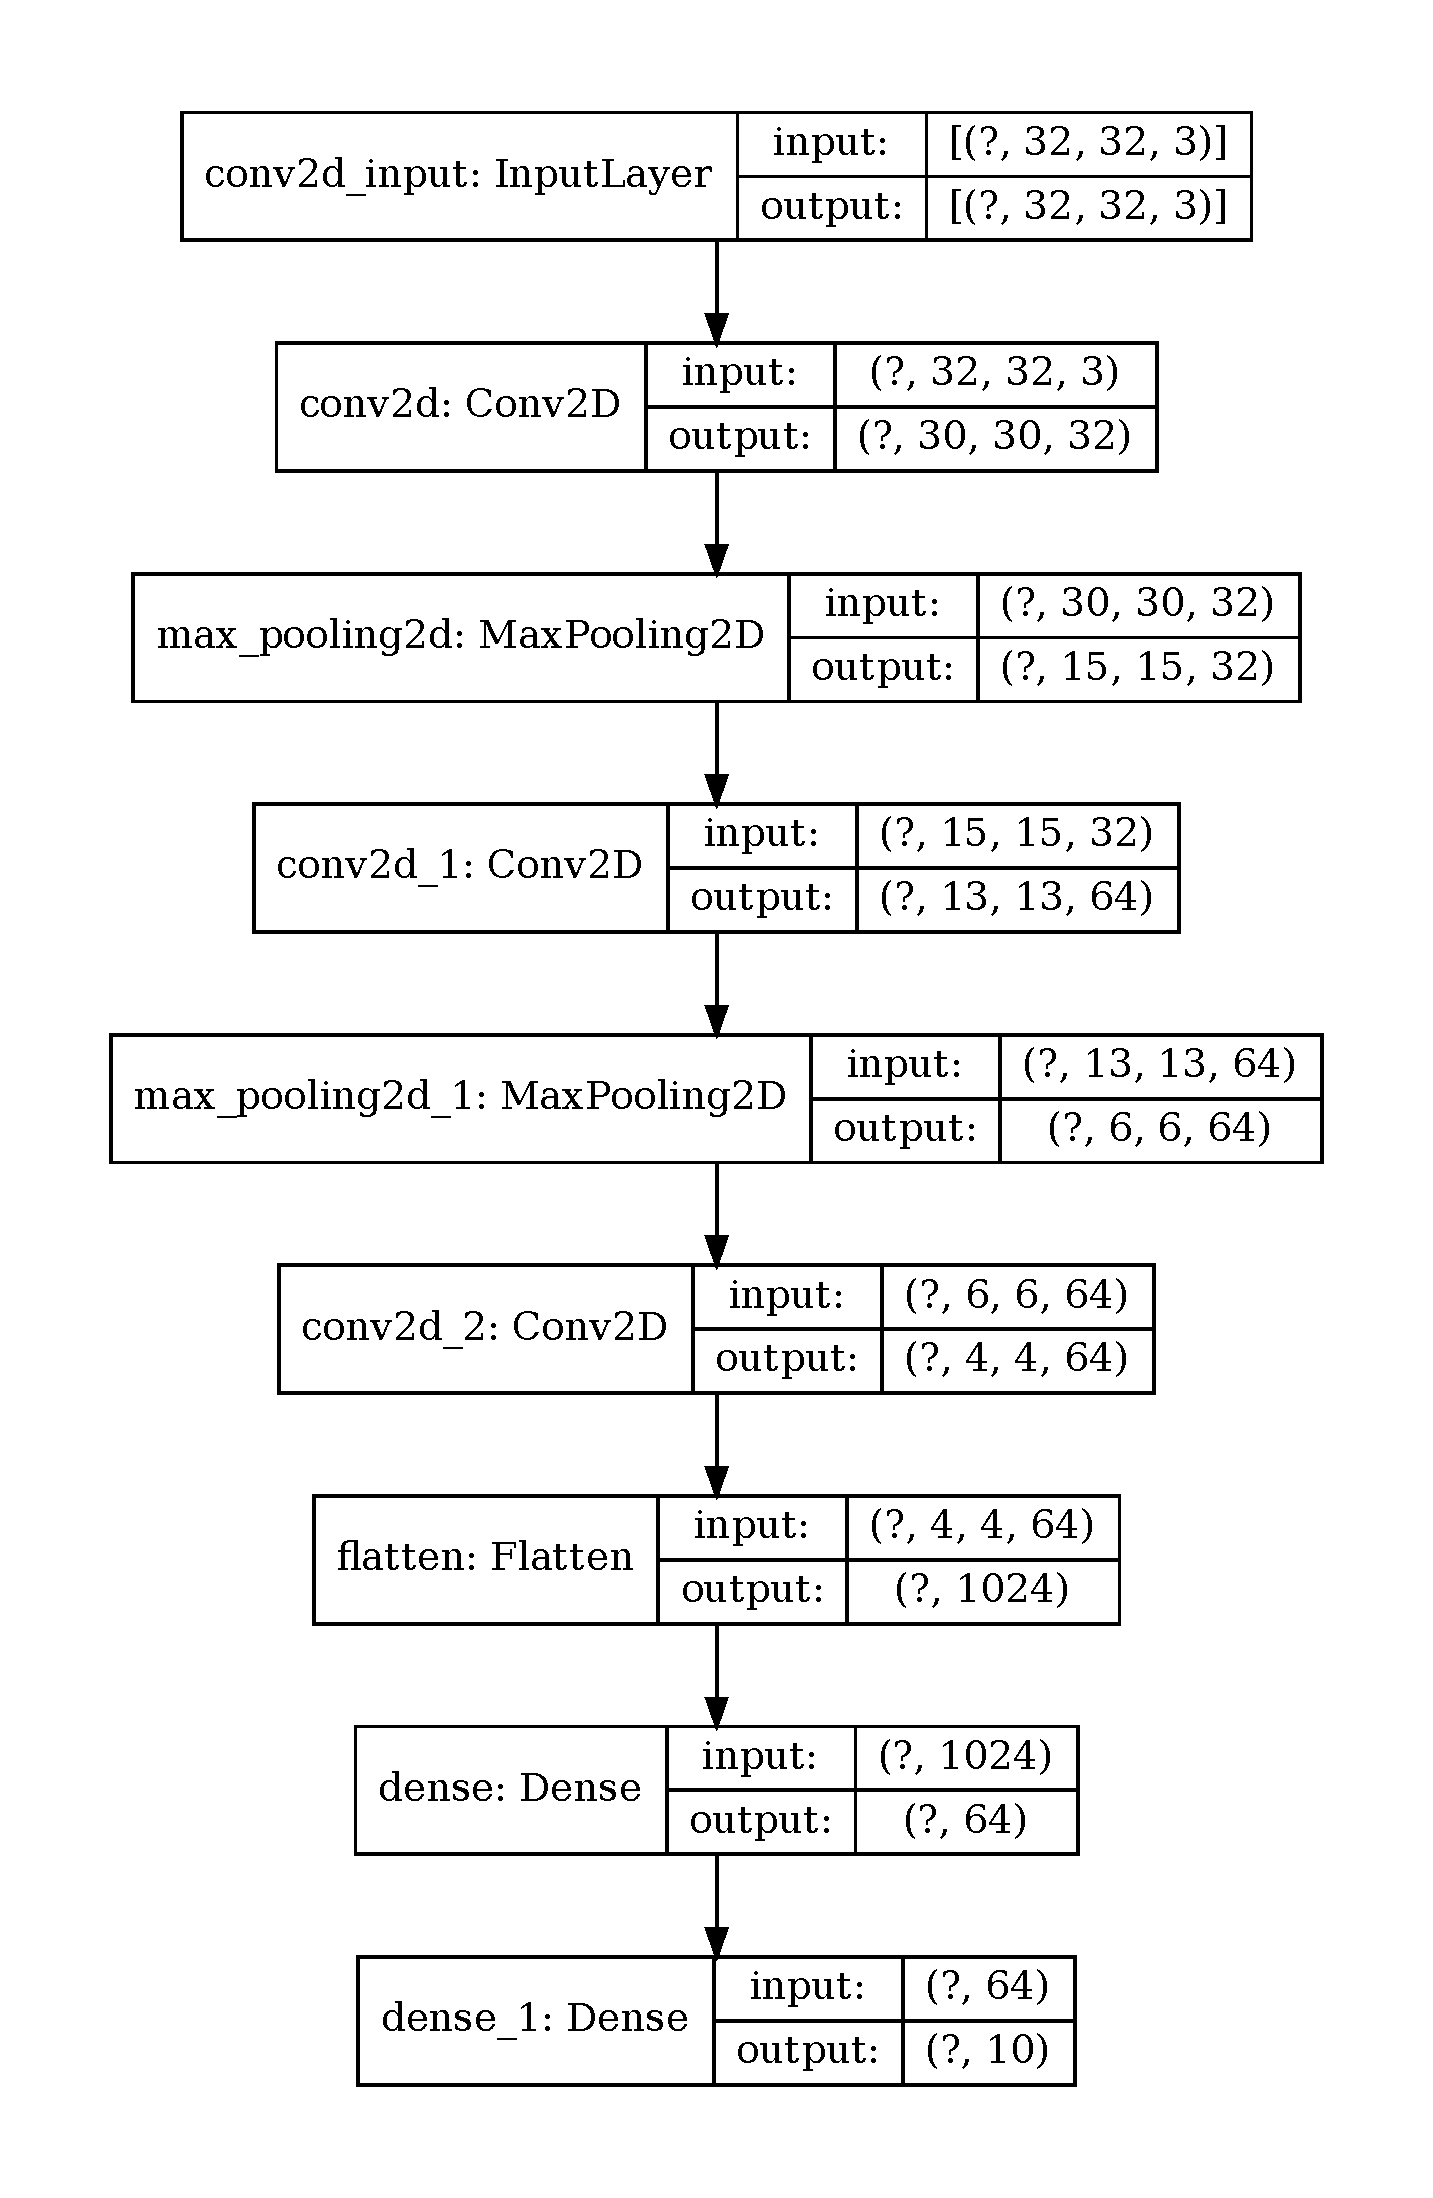
\includegraphics[trim = 0mm 19mm 0mm 19mm, clip, height=9cm]{Bilder/CUDA/cifar-model-graph-detailed.pdf}
    \caption{Structure of the neural network used}
    \label{fig:networklayers}
\end{figure}

This data is now fed again into a convolutional layer, which here is also configured with a \PYTHON{kernel\_size} of \twod{2}{2}, \cref{src:cifarlayers}, line 4, but with 64 filters. This transforms the data from \threed{15}{32} to \threed{13}{64}.

To reduce the amount of data again, another max-pooling layer is applied, which is also configured with a \PYTHON{pool\_size} of \twod{2}{2} in line 5, reducing the amount of data from \threed{13}{13}{64} to \threed{6}{6}{64}.

The last convolutional layer is then applied to this network. This, like the previous convolutional layer, works with \PYTHON{kernel\_size} \twod{2}{2} and 64 filters as per line 6. This transforms the data from \threed{6}{64} to \threed{4}{64}.

To enable classification of this information with a neural network, the so-called dense layer, the results of the convolutional layers are transformed into a vector with a flatten layer, see line 7. Due to the input size of \threed{4}{64} this results in a vector of length 1024.

The vector is fed into a Dense layer in line 8. This layer is parameterised with 64 \PYTHON{units} and the activation function \ac{relu}, which combines the 1024 input data into 64 nodes and calculates the corresponding outputs.

In the last layer, the 64 output values are passed to another Dense layer, which has been configured with 10 \PYTHON{units}. The input data are thus now reduced to 10 output data, which correspond to the classes to be identified of the data set \ac{cifar}-10.













